\section{Results and Discussion}

For the results of this Project, we represented the retrieved topic model in plots. For one we 
used a simple plot package, ggplot in R, to represent every of Lovecraft’s works in chronological 
order with their distribution of the topics. We also used the R package LDAvis to show correlations 
between the topics and use an interactive interface to see the importance of relevant terms in 
respect to a topic.\\

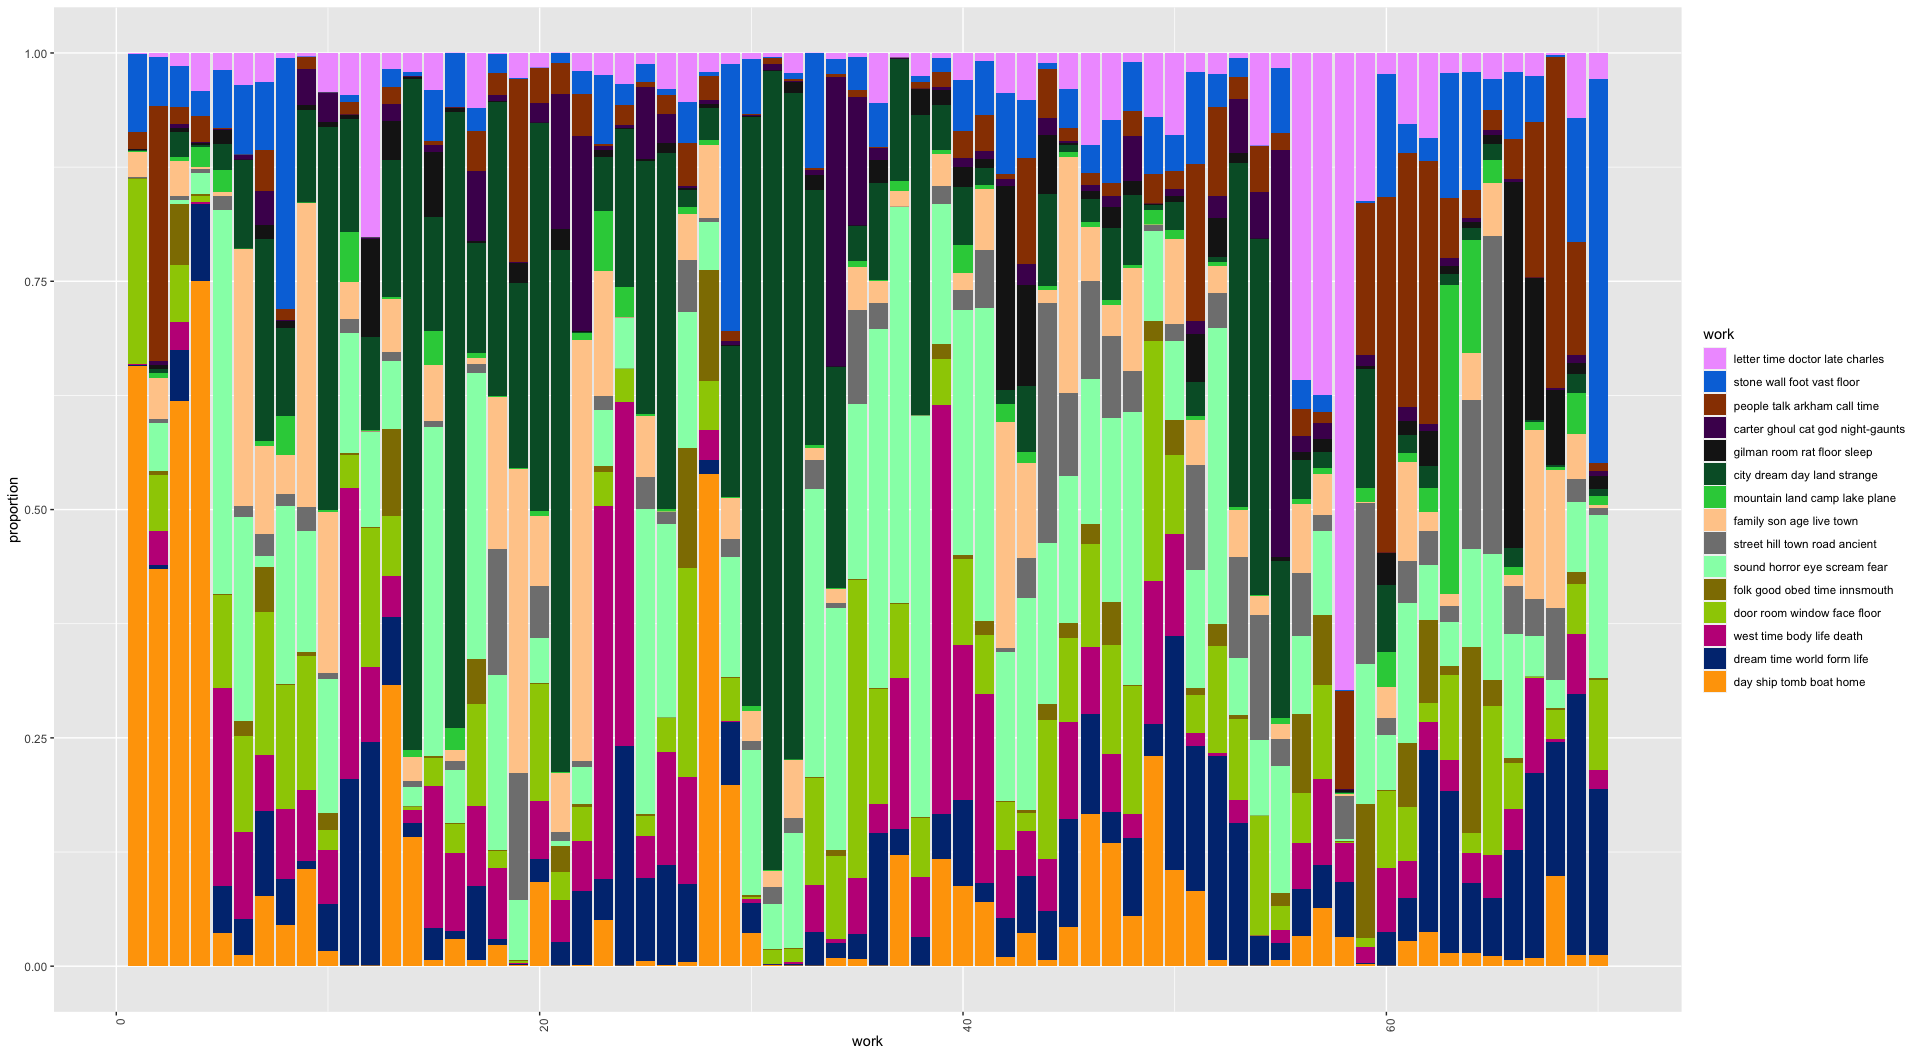
\includegraphics[width=6.5in]{/Users/ferriskleier/PECK/DigitalHumanities/Lovecraft_TopicModel/Project/images/plot_zoom.png}
Fig. 1 – The plot assigning the percentage of a topic to each story of Lovecraft

Figure 1 shows the bar chart we created to plot every of Lovecraft’s stories in chronological order 
with their percentage of the topic they share. On the x-axis you can see the number of the story. Keep in mind that we used the date Lovecraft 
wrote the story and changed unspecified dates like just a year to the January of that year. For 
the numeration of his works to compare to this figure, see stories\_list.txt. On the y-axis you 
can see the distribution in percentage. Each bar corresponds to one work and the percentage of 
a topic across each of the topics in that work. The order for each topic per entry is the same, 
it’s not ordered by percentage but by topic. On the right hand side you can find the colors for 
each topic, pink being topic 01 consisting of the words 'letter, time, doctor, late, charles'.\\

The bar chart clearly shows that some topics dominate a story and others have a fairly distributed 
amount of topics. For example the first topic in pink is highly present in some works. For the 
last work, we can confirm that ‘The Haunter of the Dark’ (written 1935) covers topic 9, 10 and 
14 really well. The bar chart also shows batches of topics for several time frames, like his 
first four works which dominated topic 15. After reviewing the topic distribution for every 
work, we were very satisfied with the results and decided to use this resulting topic model 
for further examination.\\

To put this into context with Lovecraft’s personal life, we took several events that may had 
a significant influence on him and checked for the topics of that time. We reviewed ‘An 
Epicure in the Terrible’ (Edited by David E. Schultz and S.T. Joshi) which is a perfect 
collection of essays by different authora regarding Lovecraft’s life. Topics 6 \& 14, being 
dark green and dark blue, clearly show the time Lovecraft began to write the ‘Dream Cycle’, since 
the topics represent correlate well with the stories. For work 11, ‘Beyond the Wall of Sleep’ 
(written 1919), and work 12, ‘Memory’ (written 1919), one can see the high share of topic 14, 
which just continues for later stories in the dream cycle as well. This is due to the fact that 
in 1919, Lovecraft met Lord Dunsany, who Lovecraft admired and who heavily influenced his early 
works which led to the dream cycle. The first interesting correlation between Lovecraft’s 
personal life and the graph can be seen starting from work 33, ‘The Outsider’ (written 1921), 
with topic 10 (turqoise) having a great share for some works. This may relate to the death of 
his mother in May 1921. Not only did he not write for a short period of time, but topic 10 
consists of the keywords ‘sound, horror, eye, scream, fear’ which suggests a coping to his 
mother’s death as well as the abrupt ending of the dream cycle being represented in topic 6. 
Although Lovecraft moved to Brooklyn in 1922 and married his wife, Sonia Haft Greene, there 
can be seen no clear shift in topics during the time around work 45 and following. That’s 
interesting because he did also write just one story for almost two years during that time, 
which would suggest some pattern in writing. Lovecraft started writing again when he moved 
to Red Hook, living alone because his wife worked somewhere else. It is known that Lovecraft 
despited Red Hook and was negatively standing against minorities that lived there. The only 
observable difference is, that topic 9 started to have a stable share starting from that time. 
The next observable pattern begins with 53, ‘The Silver Key’ (written 1926), which is represented 
with a higher amount of topic 6 being the topic that indicates the continuation of the dream 
cycle. This is very interesting, because Lovecraft moved back to Providence in April 1926, 
resulting from the growing homesickness and that he became increasingly depressed by his 
isolation and the masses of “foreigners” in the city. The observation of topic 6 being more 
present again due to the continuing dream cycle indicates this. For two works, ‘The Dream Quest 
of Unknown Kadath’ (written 1927, work 55) as well as ‘At the Mountains of Madness’ (written 
1931, work 63), they share the highest amount for a topic which is almost not as present in 
any other story. Our guess is, that the length of these works shifted the results a bit, but 
could also stem from the fact that Lovecraft wrote two thematically very distinct stories 
from the rest. For ‘The Dream Quest of Unknown Kadath’, it’s probably the most important 
work of the dream cycle and covers the fictional character Randolph Carter, who was supposedly 
an alter ego of Lovecraft as mentioned earlier. For ‘At the Mountains of Madness’ it’s clear 
that the terms for topic 7 certainly represent the work. The graph also suggests a high 
share of the first topic among three to four stories and a continued share of topic 3. 
The timeframe for the works covered by that topic, work 59-62 from late 1927 to 1930 
correlated to the fact that he divorced in 1929 and there may have been first signs of a shift 
in themes and motifs caused by unknown problems in his and Greenes relationship prior to the 
divorce. The topic 3 is present in some of the last works again as well as topic 5 having a 
higher share starting at work 66, ‘The Thing on the Doorstep’, which was written in summer 
of 1933 after he did not write for almost one and a half year. This indicated an observable 
shift in topics following a break from writing because of the death of his aunt Mrs. Clark in 
1932 and moving with his other aunt Mrs. Gamwell into small quarters in Providence. He was 
very close with aunt Mrs. Clark and her death could be represented in the shift starting at 
work 66. The last observation to mark is the rising share of topic 14 during his last years. 
One explanation could be that Lovecraft had a hard time selling his longer stories and concentrated 
on ghostwriting and non-fiction, resulting in fictional works he wrote being less frequent but 
more focussed on this topic.
